\documentclass[11pt, a4paper]{article}

\usepackage[top = 1 in, bottom = 1 in, left = 0.8 in, right = 0.8 in]{geometry}

\usepackage{amsmath, amssymb, amsfonts}
\usepackage{enumerate}
\usepackage{multirow}
\usepackage{hhline}
\usepackage{array}
\usepackage{longtable}
\usepackage{graphicx}
\usepackage{tabularray}
\usepackage{undertilde}
\usepackage{dingbat}
\usepackage{fontawesome5}
\usepackage{xcolor}
\usepackage[colorlinks=true, linkcolor=blue, urlcolor=red]{hyperref}
\usepackage{tasks}
\usepackage{bbding}
\usepackage{twemojis}
% how to use bull's eye ----- \scalebox{2.0}{\twemoji{bullseye}}
\usepackage{customdice}
% how to put dice face ------ \dice{2}
\usepackage{bclogo}
\usepackage{subcaption}


\definecolor{col1}{HTML}{EB6C0E}
\definecolor{col2}{HTML}{D503FF}


\title{MSMS 301 - Time Series}
\author{Ananda Biswas}
\date{\today}


\begin{document}

\maketitle

\tableofcontents

\newpage

\begin{flushright}
\textcolor{col2}{@ 01.08.2025, Friday}
\end{flushright}

\section{Moving Average Process}

Suppose $\{Z_t\}$ is a purely random process with mean $0$ and variance $\sigma^2$. A process $\{X_t\}$ derived as a \underline{weighted} sum of \textcolor{col1}{\textbf{present and past $\mathbf{q}$}} white noises is said to be a Moving Average Process of order $q$ (abbreviated to $MA(q)$).

\begin{equation}\label{maq}
X_t = \beta_0 Z_t + \beta_1 Z_{t-1} + \ldots + \beta_q Z_{t-q}
\end{equation}

where all $\beta_i$'s are constants. The $Z$'s are usually scaled so that $\beta_0 = 1$. \\[0.5em]

It immediately follows

\begin{itemize}
\item $E(X_t) = 0$ $\forall t$ as $E(Z_t) = 0$ $\forall t$

\item $Var(X_t) = \sigma^2 \sum \limits_{i = 0}^{q} \beta_{i}^{2}$ $\forall t$ as $Z_t \overset{ind}{\sim} \text{variance } = \sigma^2$ $\forall t$.
\end{itemize}

\subsection{MA(1) Process}

With $Z_t \sim \text{White Noise }(0, \sigma^2)$, the first order moving average process $\{X_t\}$ is defined as

\begin{align}
X_t &= \beta_0 Z_t + \beta_1 Z_{t-1}; \,\, \beta_0 = 1 \\[0.25em]
\text{or } X_t &= Z_t + \theta Z_{t-1}
\end{align}

where $\theta \in \mathbb{R}$ (as the process is finite, $\theta$ is free to be any real constant).\\


Clearly $E(X_t) = 0$ $\forall t$ and $Var(X_t) = \sigma^2 (1 + \theta^2)$. \\[0.25em]

Now 
\begin{align*}
\gamma(h) &= cov(X_t, X_{t+h}) \\[0.25em]
&= cov(Z_t + \theta Z_{t-1}, Z_{t+h} + \theta Z_{t+h-1}) \\[0.25em]
&= cov(Z_t, Z_{t+h}) + \theta \cdot cov(Z_t, Z_{t+h-1}) + \theta \cdot  cov(Z_{t-1}, Z_{t+h}) + \theta^2 \cdot cov(Z_{t-1}, Z_{t+h-1}) \\[0.25em]
&= \begin{cases}
\sigma^2 (1 + \theta^2), \,\, h = 0 \\[0.25em]
\theta \sigma^2 , \,\, h = \pm 1 \\[0.25em]
0, \,\, h = \pm 2, \pm 3, \pm 4, \ldots
\end{cases}
\end{align*}

Then
\begin{align*}
\rho(h) &= \dfrac{\gamma(h)}{\gamma(0)} \\[0.35em]
&= \begin{cases}
1, \,\, h = 0 \\[0.25em]
\dfrac{\theta}{1 + \theta^2}, \,\, h = \pm 1 \\[0.5em]
0, \,\, h = \pm 2, \pm 3, \pm 4, \ldots
\end{cases}
\end{align*}

\smallpencil \hspace{0.1cm} So, for MA(1) process, the autocorrelation function vanishes after lag 1. This is an identifier for MA(1) process.

\subsection{MA(q) Process}

$MA(q)$ process as in (\ref{maq}) can be written as $X_t = \sum \limits_{i = 0}^{q} \beta_i Z_{t-i}$. \\[0.25em]

Then
\begin{align*}
\gamma(h) &= cov(X_t, X_{t+h}) \\[0.25em]
&= cov \left(\sum \limits_{i = 0}^{q} \beta_i Z_{t-i}, \sum \limits_{j = 0}^{q} \beta_j Z_{t+h-j} \right) \\[0.25em]
&= cov \left(\sum \limits_{i = 0}^{q} \beta_i Z_{t-i}, \sum \limits_{s = -h}^{q-h} \beta_{s+h} Z_{t-s} \right) \,\,\,\, [s = j-h] \\[0.25em]
&= cov \left(\sum \limits_{i = 0}^{q} \beta_i Z_{t-i}, \sum \limits_{i = -h}^{q-h} \beta_{i+h} Z_{t-i} \right) \,\,\, [\text{runner } s \text{ is just a dummy variable}]\\[0.25em]
&= \sum \limits_{i = 0}^{q - h} \beta_{i}\beta_{i+h} \cdot cov(Z_{t-i}, Z_{t-i}) \\[0.25em]
&= \sigma^2 \sum \limits_{i = 0}^{q - h} \beta_{i}\beta_{i+h} \\[0.25em]
&= \begin{cases}
\sigma^2 \sum \limits_{i = 0}^{q - h} \beta_{i}\beta_{i+h}, \,\, h = 0, 1, \ldots, q \\[0.25em]
0, \,\, h > q \\[0.5em]
\gamma(-h), \,\, h < 0
\end{cases}
\end{align*}

\vspace{0.25cm}

Consequently

\begin{align*}
\rho(h) &= \dfrac{\gamma(h)}{\gamma(0)} \\[0.35em]
&= \begin{cases} 
\dfrac{\sum \limits_{i = 0}^{q - h} \beta_{i}\beta_{i+h}}{\sum \limits_{i = 0}^{q} \beta_{i}^{2}}, \,\, h = 0, 1, \ldots, q \\[1em]
0, \,\, h > q \\[0.5em]
\rho(-h), \,\, h < 0
\end{cases}
\end{align*}

\smallpencil \hspace{0.1cm} It can be seen from the above expression that ACF becomes $0$ at lag $k > q$. It shows that ACF of MA process cuts off at lag $q$ which is a special characteristics of MA$(q)$ process.

\vspace{0.5cm}

\begin{flushright}
\textcolor{col2}{@ 03.08.2025, Sunday (Yesss !! On a goddaamn Sunday !! \scalebox{1.5}{\twemoji{smiling face with tear}})}
\end{flushright}

\bclampe \hspace{0.1cm} \underline{Random Cosine Curve} : Consider a stochastic process $\{X_t\}$ given by $$X_t = \cos \left( 2\pi \left( \dfrac{t}{12} + \Phi \right) \right). \,\,\, t = 0, \pm 1, \pm 2, \ldots$$
where $\Phi \sim U(0, 1)$. Find $E(X_t)$ and $Var(X_t)$.

\section{Autoregressive Process}

\subsection{AR(1) Process}

The first-order autoregressive process $\{X_t\}$ is defined as

\begin{equation}\label{ar1}
X_t = \alpha X_{t-1} + Z_t \,\,\, t = 0, \pm 1, \pm 2, \ldots
\end{equation}

where $Z_t$'s are White Noise with mean $0$ and variance $\sigma^2$; $\alpha \in \mathbb{R}$, constant. \\

Notice (\ref{ar1}) reduces to a random walk model for $\alpha = 1$. \\

We may write (\ref{ar1}) as $X_t = \alpha BX_{t} + Z_t \,\,\, \text{where } B \text{ is a backshift operator with } BX_t = X_{t-1}$. \\

Then $(1 - \alpha B) X_t = Z_t$ so that

\begin{align}\label{ar1inftysum}
X_t &= (1 - \alpha B)^{-1} Z_t \nonumber \\
&= (1 + \alpha B + \alpha^2 B^2 + \alpha^3 B^3 + \ldots) Z_t \nonumber \\
&= Z_t + \alpha Z_{t-1} + \alpha^2 Z_{t-2} + \alpha^3 Z_{t-3} + \ldots \nonumber \\
&= \sum \limits_{j = 0}^{\infty} \alpha^j Z_{t-j} \,\,\, \text{provided the sum exists } i.e. \,\, |\alpha| < 1
\end{align}

Using (\ref{ar1inftysum}), $E(X_t) = 0$, $t = 0, \pm 1, \pm 2, \ldots$ \\

And $Var(X_t) = \sigma^2 \sum \limits_{j = 0}^{\infty} \alpha^{2j} = \dfrac{\sigma^2}{1 - \alpha^2}$, provided $|\alpha| < 1$. \\

Then
\begin{align*}
\gamma(h) &= cov(X_t, X_{t+h}) \\[0.25em]
&= cov\left(\sum \limits_{j = 0}^{\infty} \alpha^j Z_{t-j}, \sum \limits_{j = 0}^{\infty} \alpha^j Z_{t+h-j}\right) \\[0.25em]
&= cov \left(\sum \limits_{j = 0}^{\infty} \alpha^j Z_{t-j}, \sum \limits_{k = - h}^{\infty} \alpha^{k+h} Z_{t-k} \right), \,\, \text{taking } k = j - h \\[0.25em]
&= \sigma^2 \sum \limits_{j = 0}^{\infty} \alpha^j \alpha^{j+h} \\[0.25em]
&= \sigma^2 \alpha^h \sum \limits_{j = 0}^{\infty} \alpha^{2j} \\[0.25em]
&= \dfrac{\sigma^2 \alpha^h}{1 - \alpha^2} \text{ provided } |\alpha| < 1, h \geq 0
\end{align*}
\\
Note that $\gamma(h)$ does not depend on $t$. So AR(1) model is \underline{weak stationary} only if $|\alpha| < 1$. \\

Consequently
\begin{align*}
\rho(h) &= \dfrac{\gamma(h)}{\gamma(0)} \\[0.25em]
&= \begin{cases} 
1, \,\, h = 0 \\
\alpha^h, \,\, h = 1, 2, \ldots \\
\rho(-h), \,\, h = -1, -2, \ldots
\end{cases} \\[0.25em]
&= \alpha^{|h|}, \,\, h = \pm 1, \pm 2, \ldots
\end{align*}

Multiplying $X_{t-k}$ on both sides of (\ref{ar1}) and taking expectation we get

\begin{align}\label{ar1diffeqn}
E(X_t \cdot X_{t-h}) &= \alpha E(X_{t-1} \cdot X_{t-h}) + E(Z_{t} \cdot X_{t-h}),  \nonumber \\[0.25em]
\Rightarrow \gamma(h) &= \alpha \, \gamma(h-1)
\end{align}

Remember $Z_t$, $X_{t-h}$ are independent and $E(X_t) = 0$ $\forall t$. Also, using (\ref{ar1inftysum}), $cov(Z_{t}, X_{t-h}) = 0$.\\

Following (\ref{ar1diffeqn}) we have
\begin{align}\label{ar1reqrel}
\gamma(1) &= \alpha \, \gamma(0) \nonumber \\[0.25em]
\gamma(2) &= \alpha^2 \, \gamma(0) \nonumber \\[0.25em]
&\vdots \nonumber \\[0.25em]
\gamma(h) &= \alpha^h \gamma(0)
\end{align}

On dividing both sides of (\ref{ar1reqrel}) by $\gamma(0)$, we get $$\rho(h) = \alpha^{|h|}, \,\, h = 0, \pm 1, \pm 2, \ldots$$ \\

\bclampe \hspace{0.1cm} Find ACVF \& ACF and draw the ACF plot for the following $AR(1)$ processes.
\begin{enumerate}[(i)]
\item $X_t = 0.35 \, X_{t-1} + Z_t$
\item $X_t = 0.85 \, X_{t-1} + Z_t$
\item $X_t = -0.35 \, X_{t-1} + Z_t$
\end{enumerate}

\bcplume \hspace{0.1cm} The ACVFs and ACFs are as follows.
\begin{enumerate}[(i)]
\item $\gamma(h) = 0.8775 \cdot \sigma^2 \, 0.35^{|h|}$, $\rho(h) = 0.35^{|h|}$ $\forall h = 0, \pm 1, \pm 2, \ldots$
\item $\gamma(h) = 0.2775 \cdot \sigma^2 \, 0.85^{|h|}$, $\rho(h) = 0.85^{|h|}$ $\forall h = 0, \pm 1, \pm 2, \ldots$
\item $\gamma(h) = 0.8775 \cdot \sigma^2 \, (-0.35)^{|h|}$, $\rho(h) = (-0.35)^{|h|}$ $\forall h = 0, \pm 1, \pm 2, \ldots$
\end{enumerate}

\newpage

\begin{figure}[h!]
  \centering
  \begin{subfigure}[t]{0.3\textwidth}
    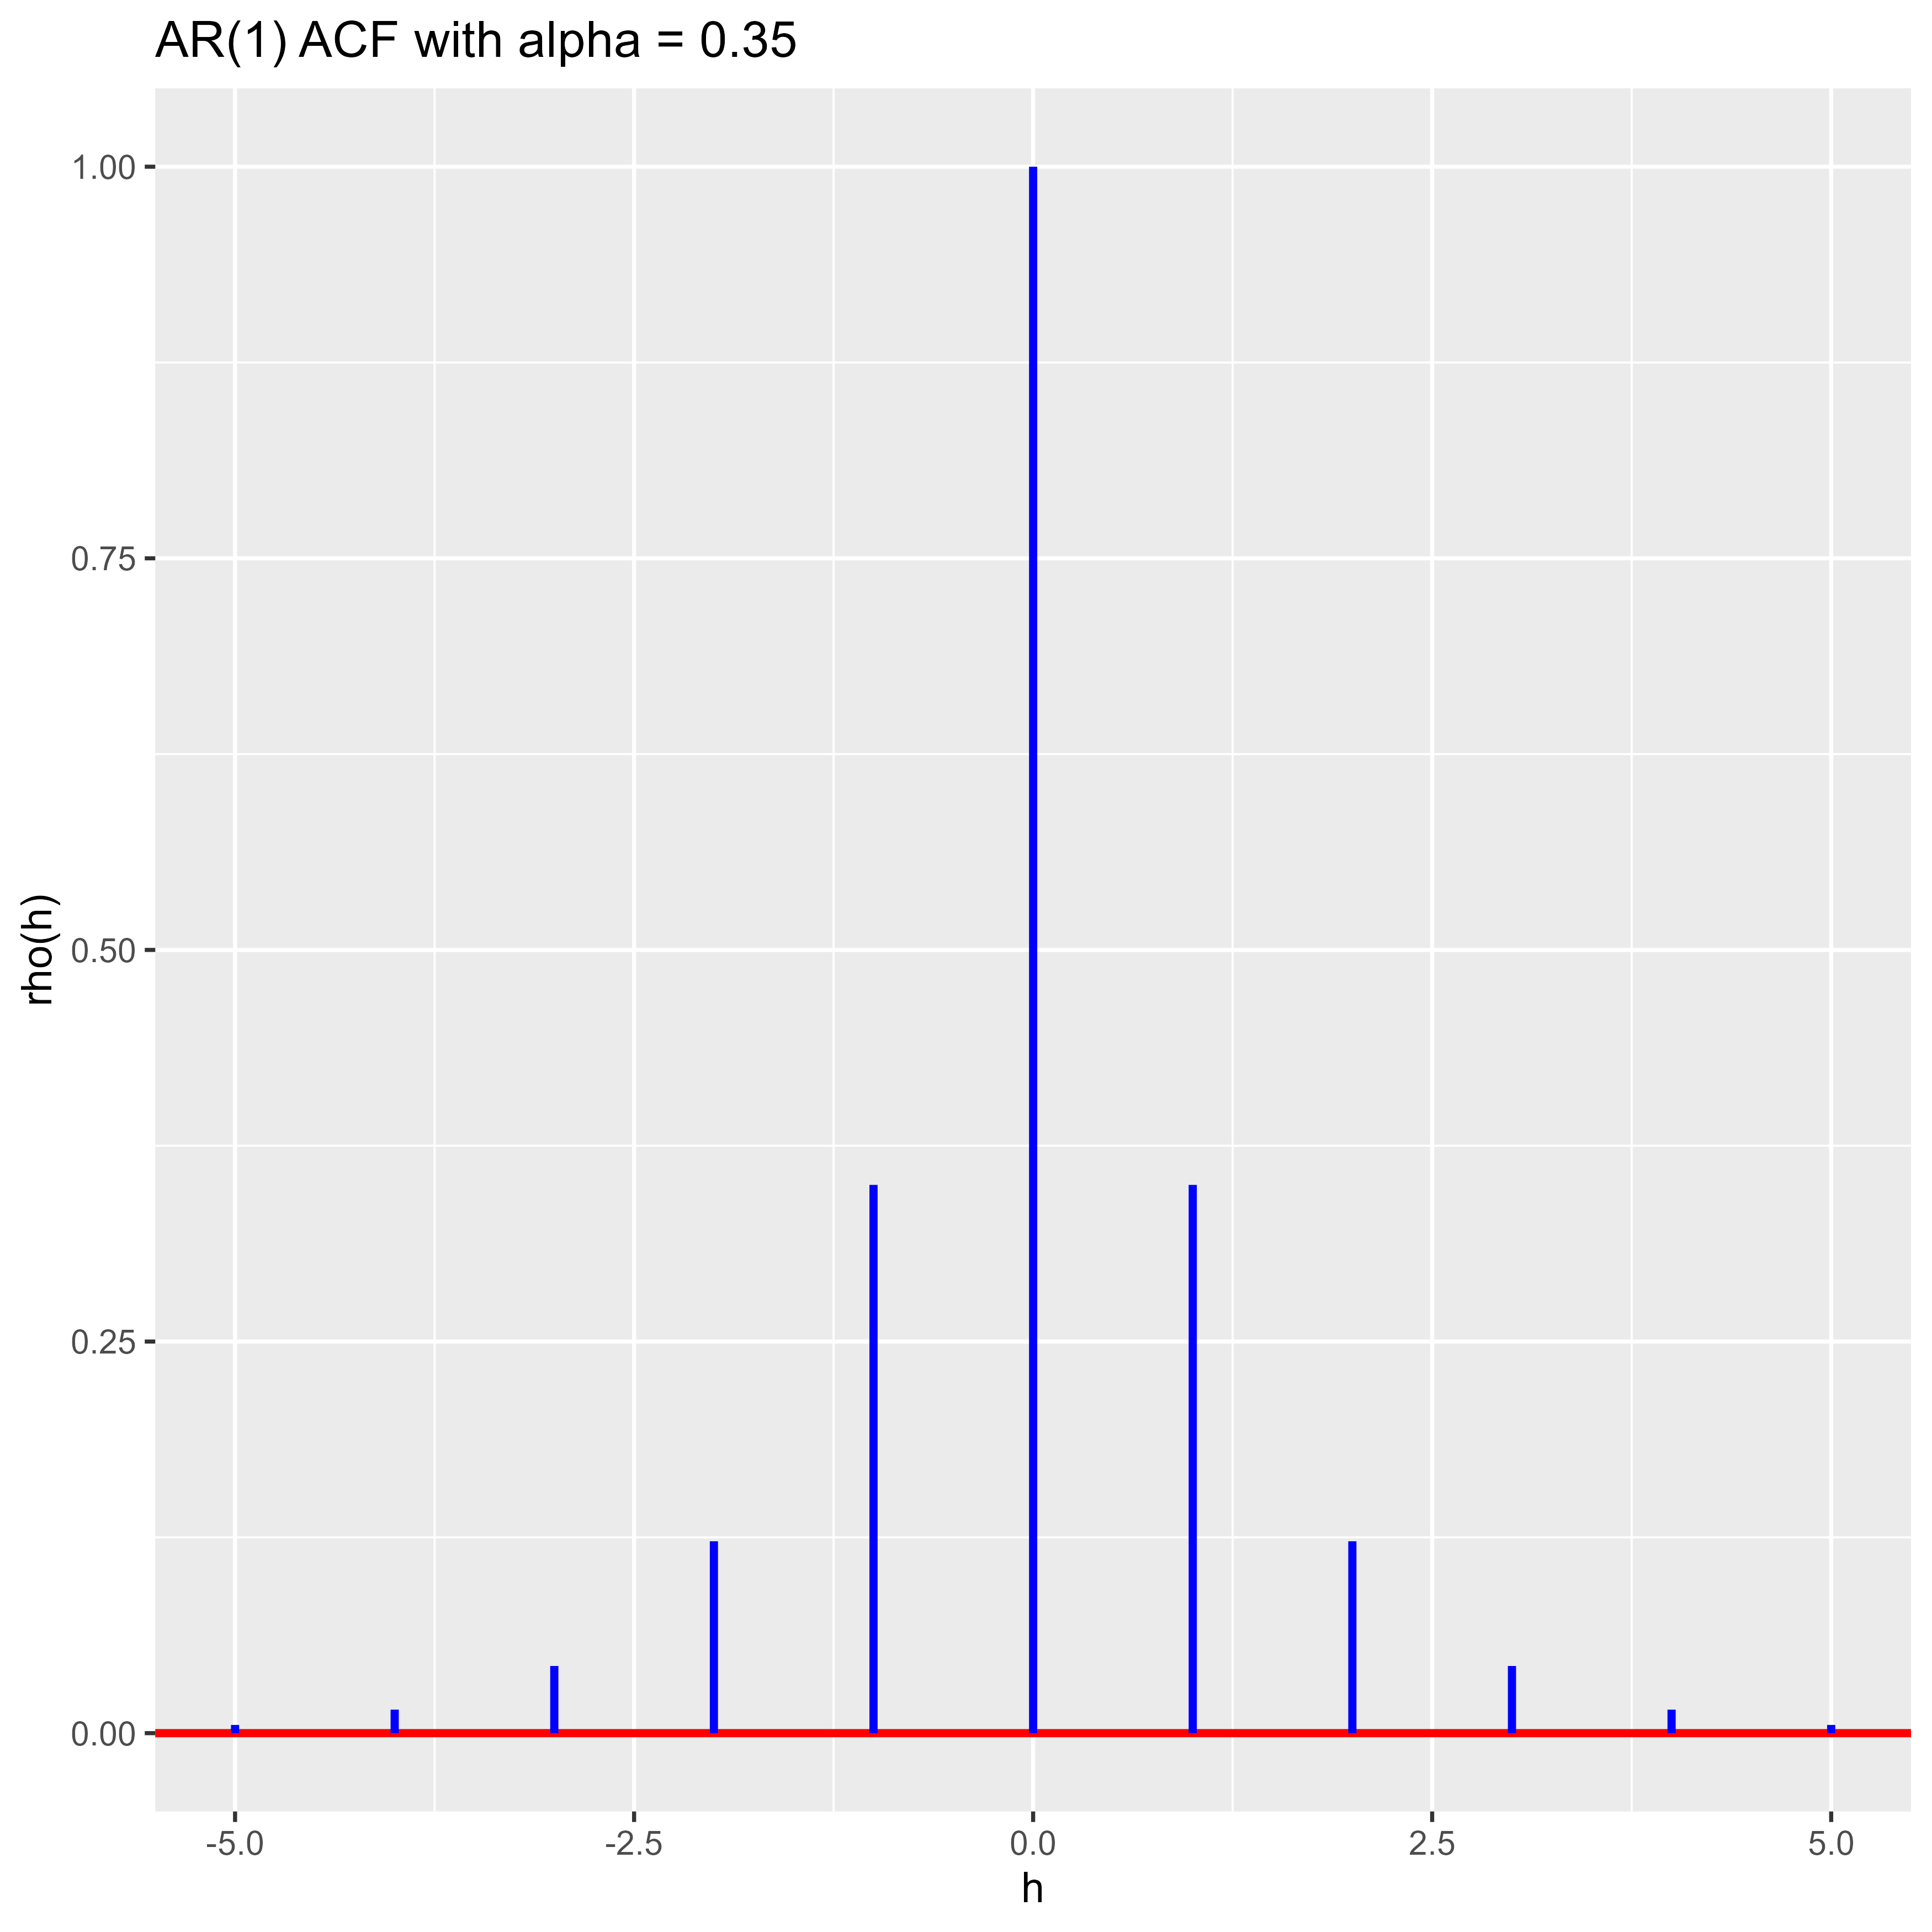
\includegraphics[width=\linewidth]{alpha_0.35.png}
    \caption*{(i)}
  \end{subfigure}
  \hfill
  \begin{subfigure}[t]{0.3\textwidth}
    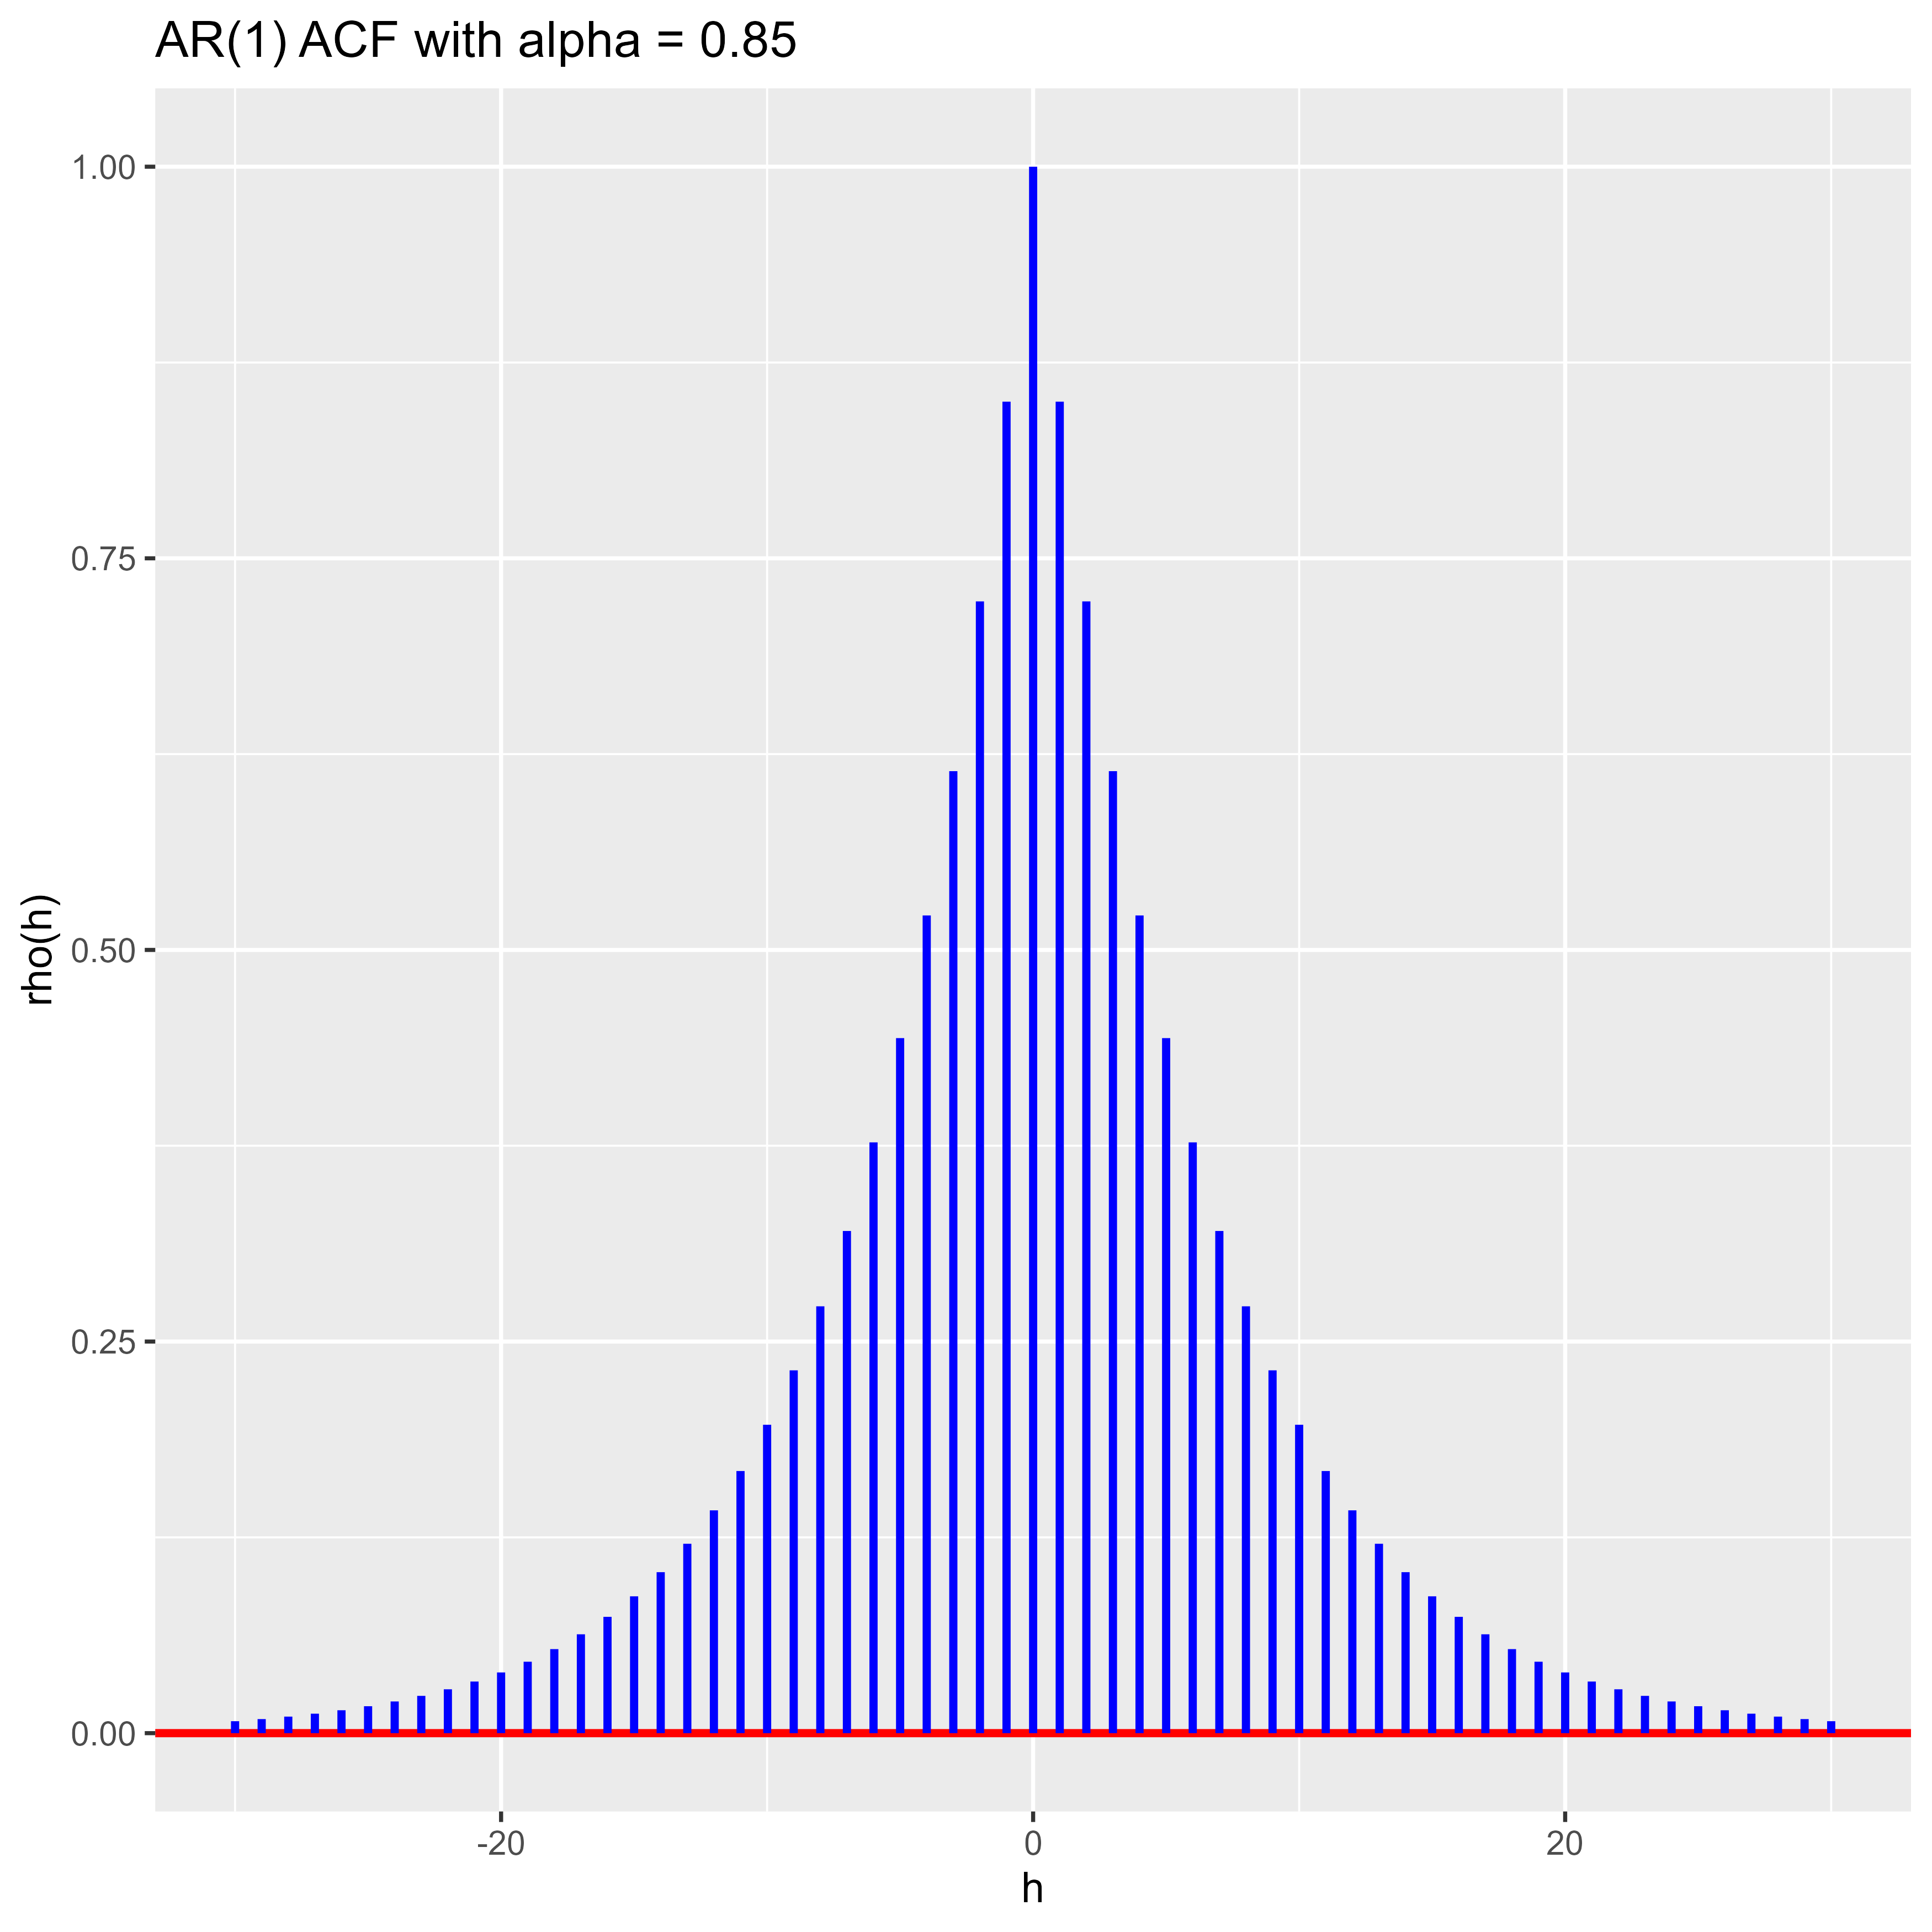
\includegraphics[width=\linewidth]{alpha_0.85.png}
	\caption*{(ii)}
  \end{subfigure}
  \hfill
  \begin{subfigure}[t]{0.3\textwidth}
    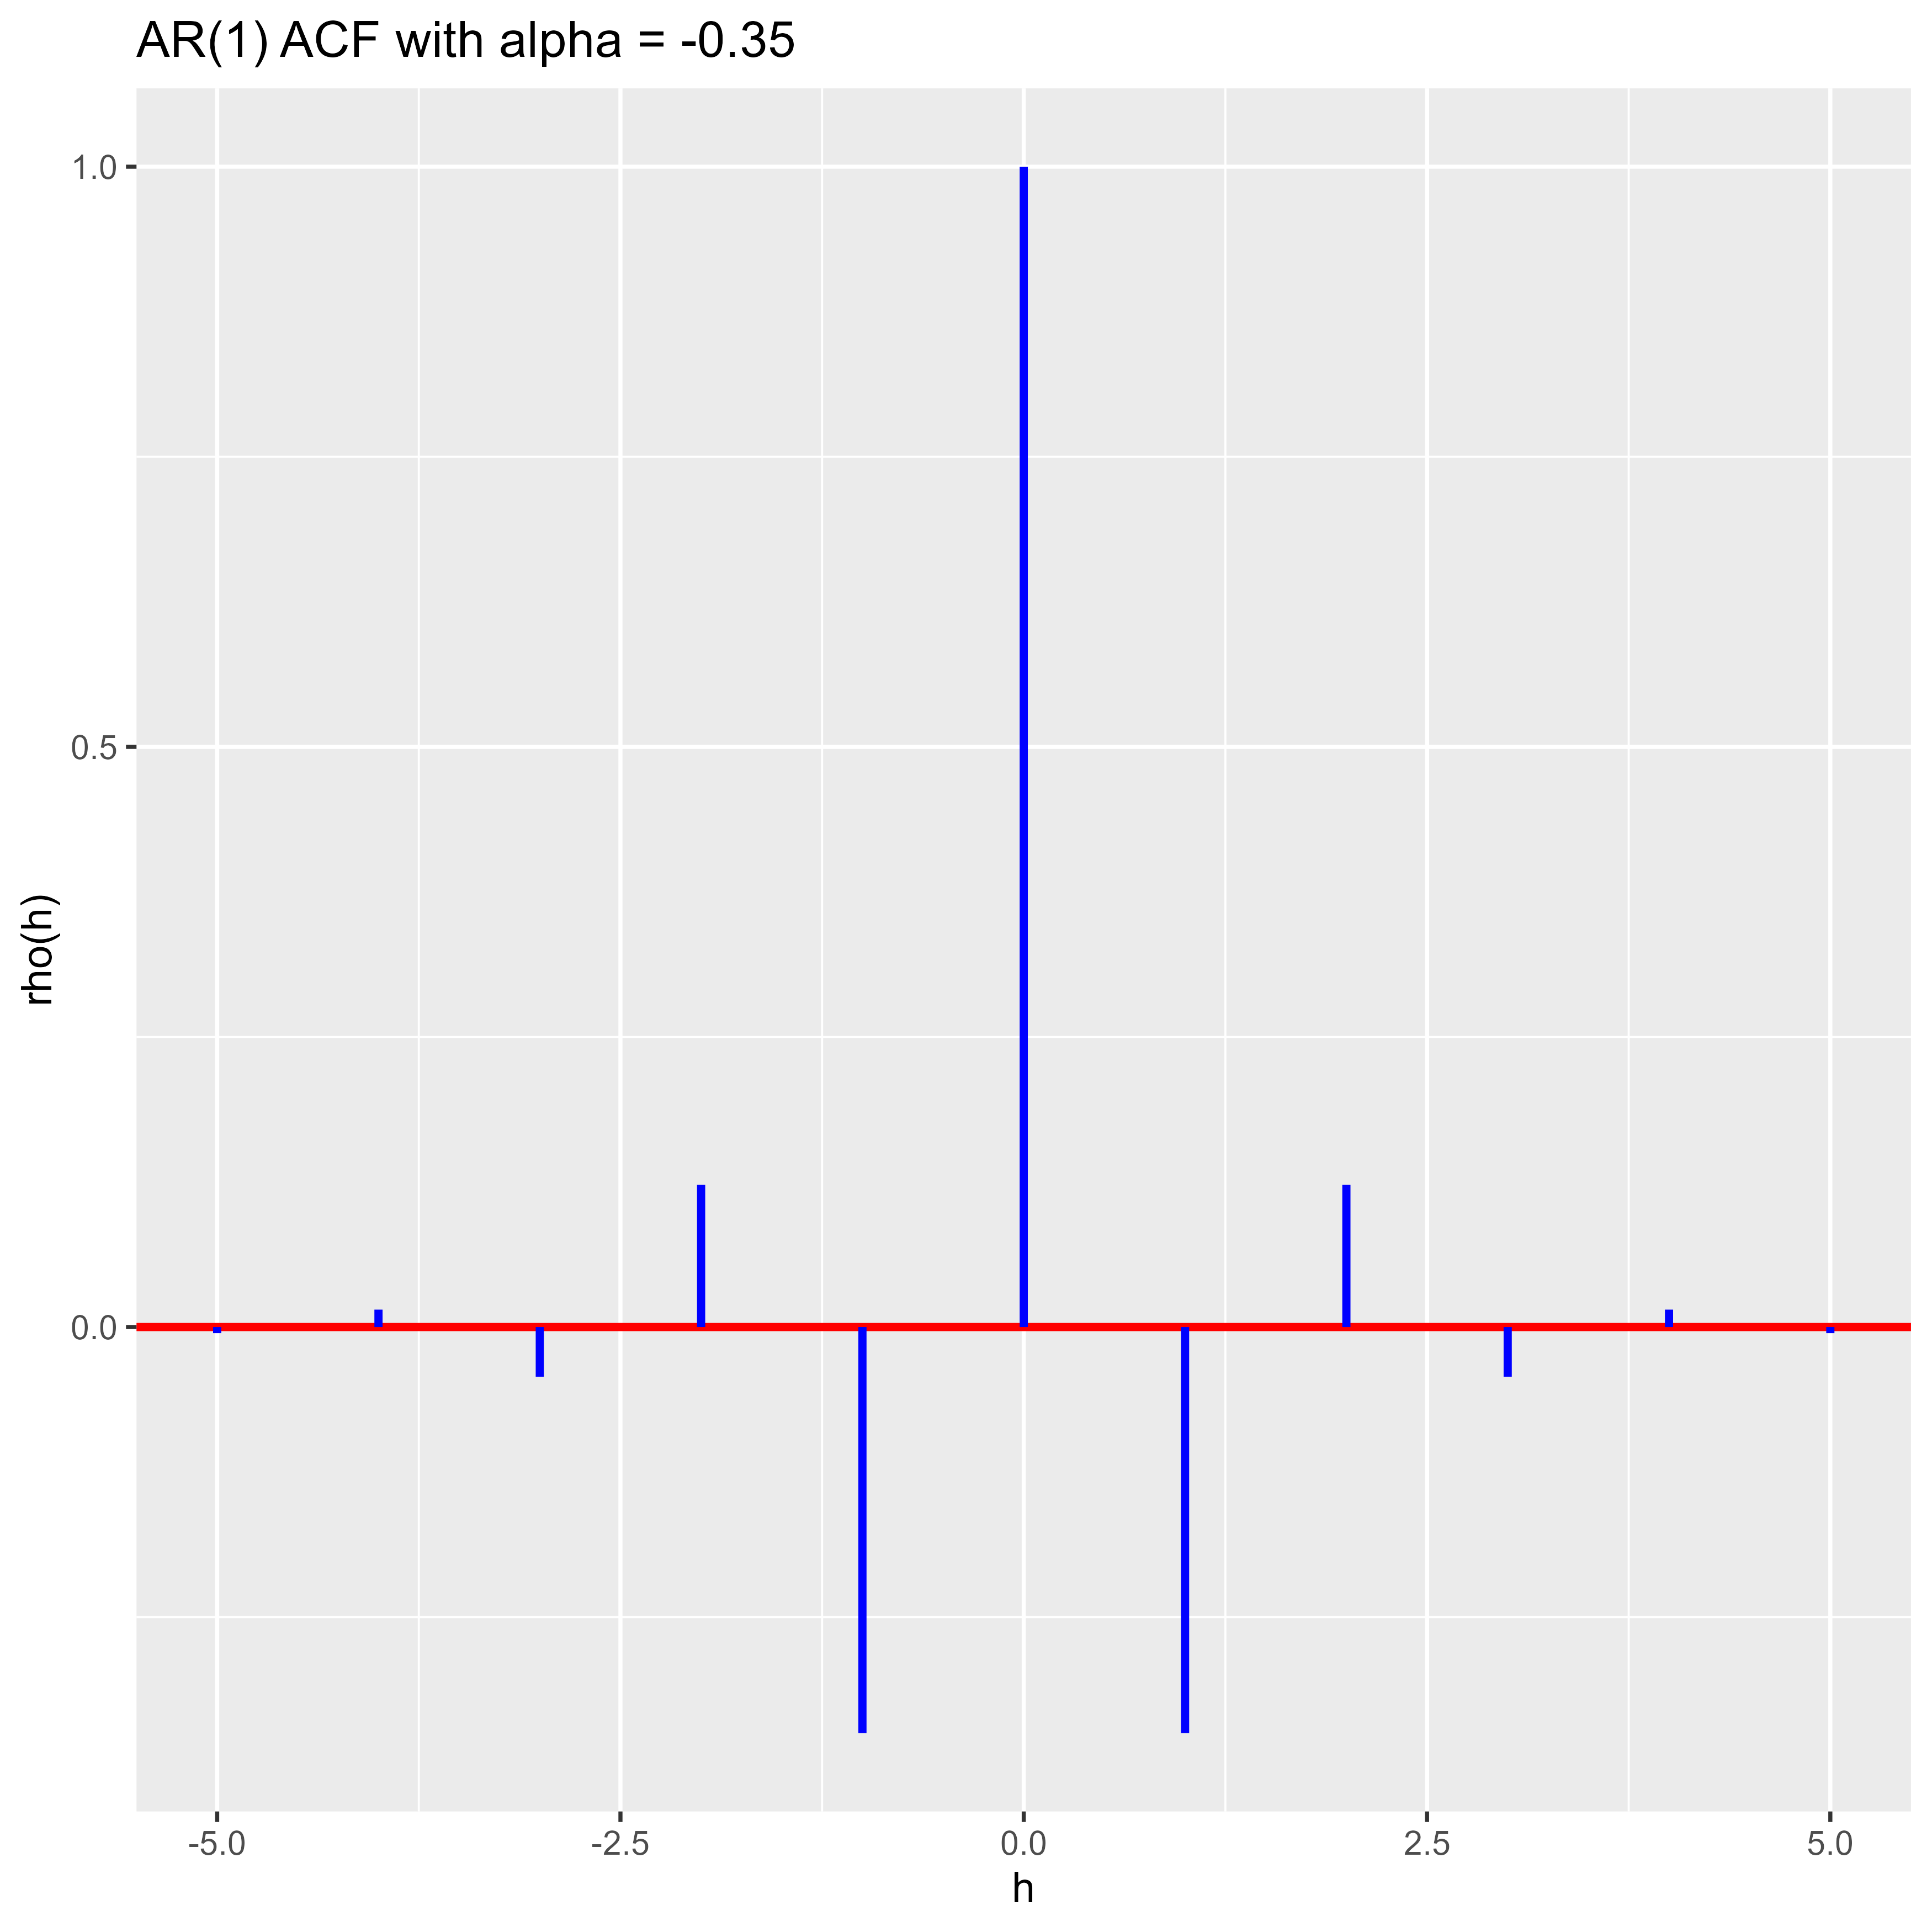
\includegraphics[width=\linewidth]{alpha_negative_0.35.png}
    \caption*{(iii)}
  \end{subfigure}
\end{figure}

\subsection{AR(2) Process}
\end{document}